\begin{figure}
\begin{subfigure}{0.3\linewidth}
	\centering
	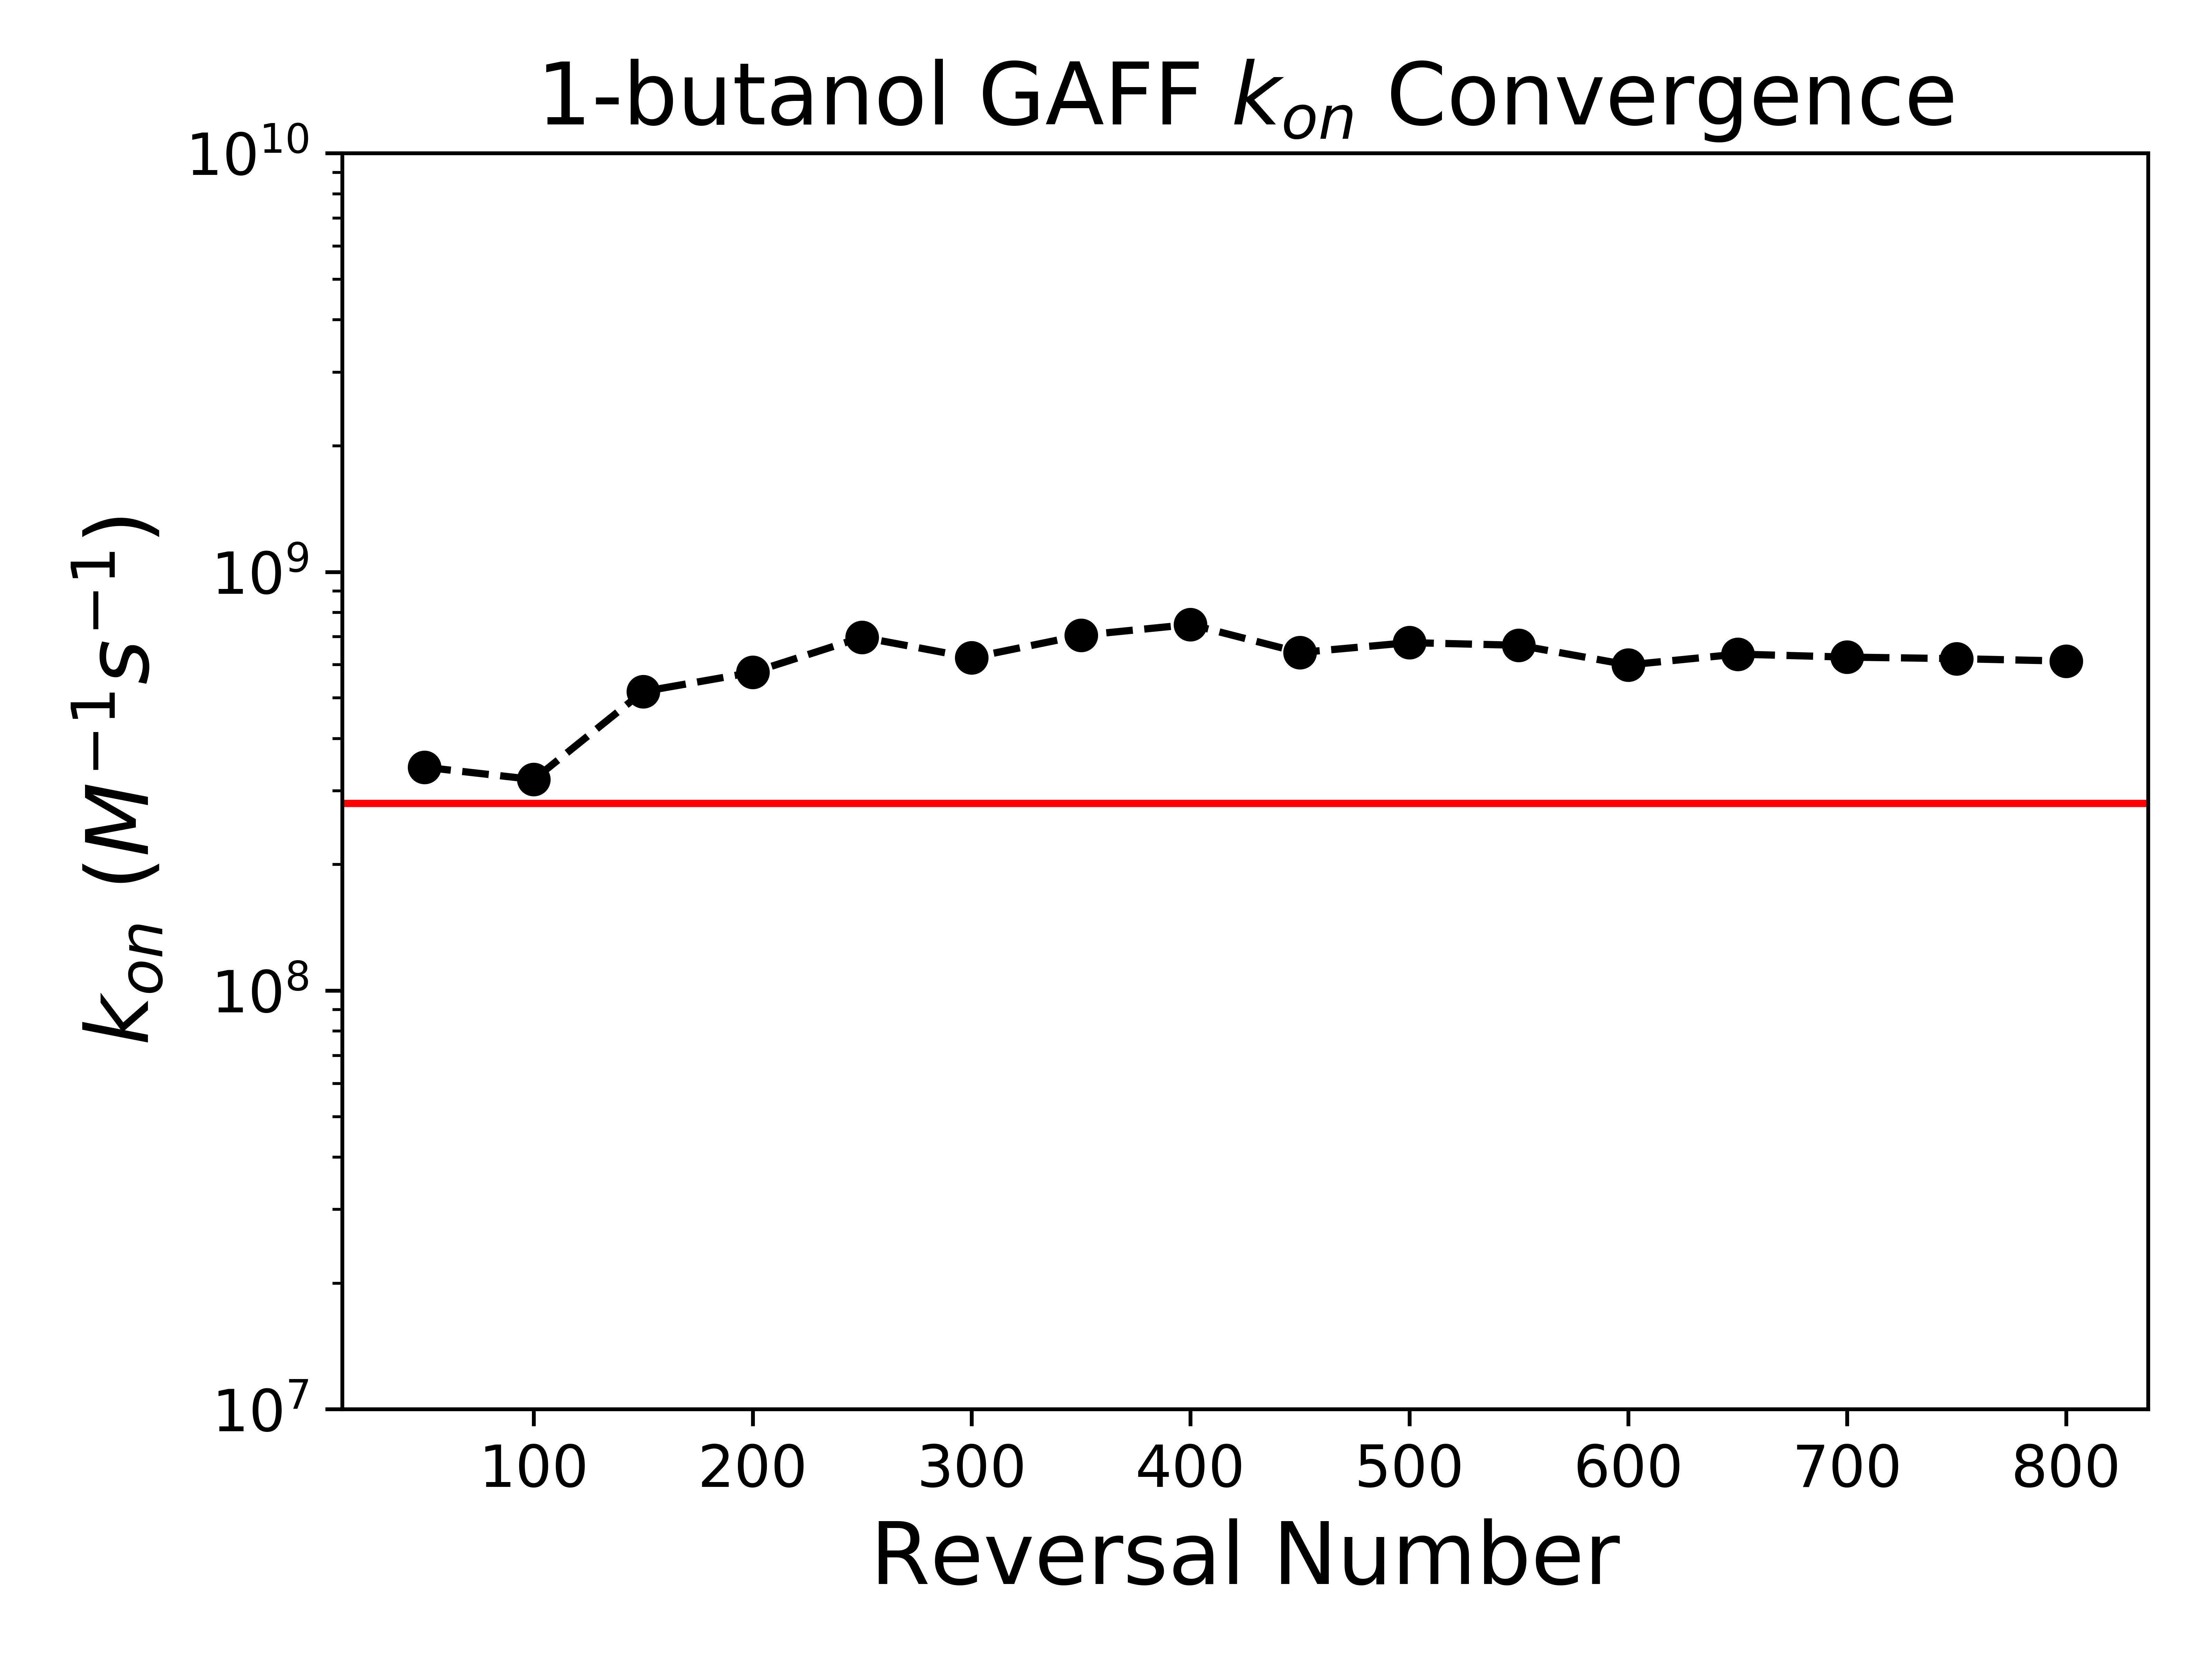
\includegraphics[width=\linewidth]{high_res_images/gaff_rate_conv_images/1-butanol_gaff_on_conv.png}
	\end{subfigure}%
\begin{subfigure}{0.3\linewidth}
		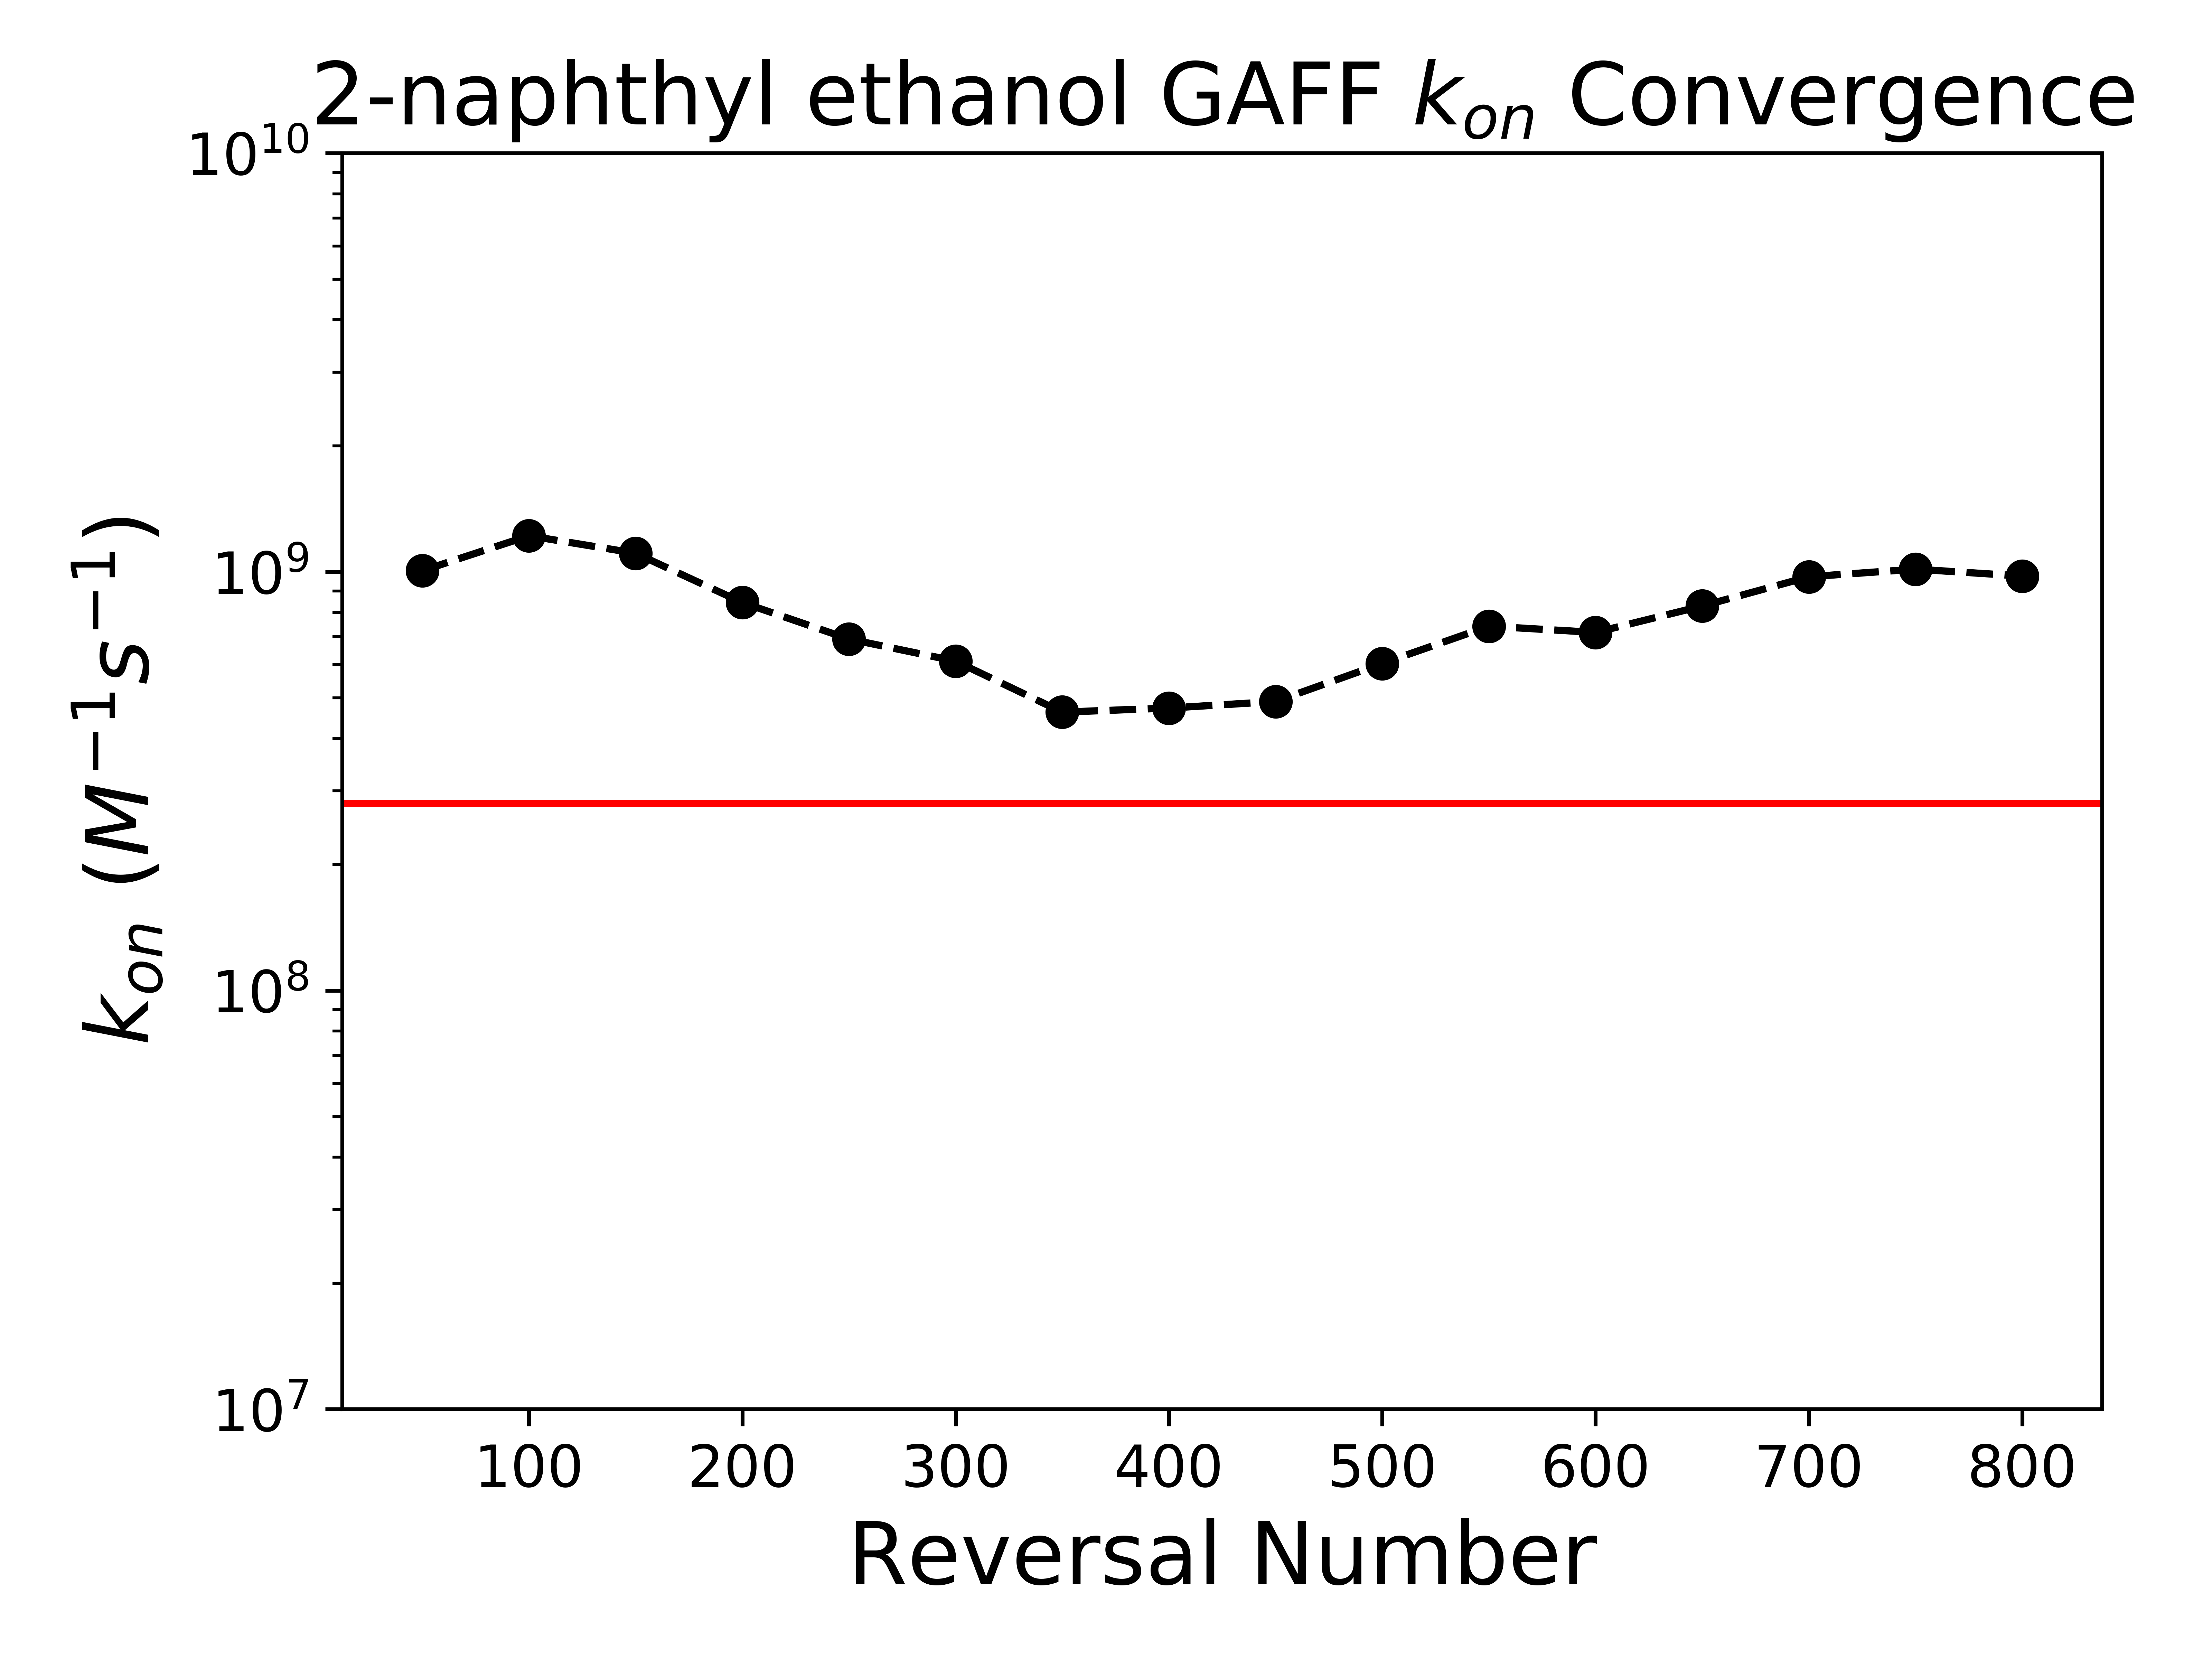
\includegraphics[width=\linewidth]{high_res_images/gaff_rate_conv_images/2-naphthylethanol_gaff_on_conv.png}
\end{subfigure}%
	\begin{subfigure}{0.3\linewidth}
		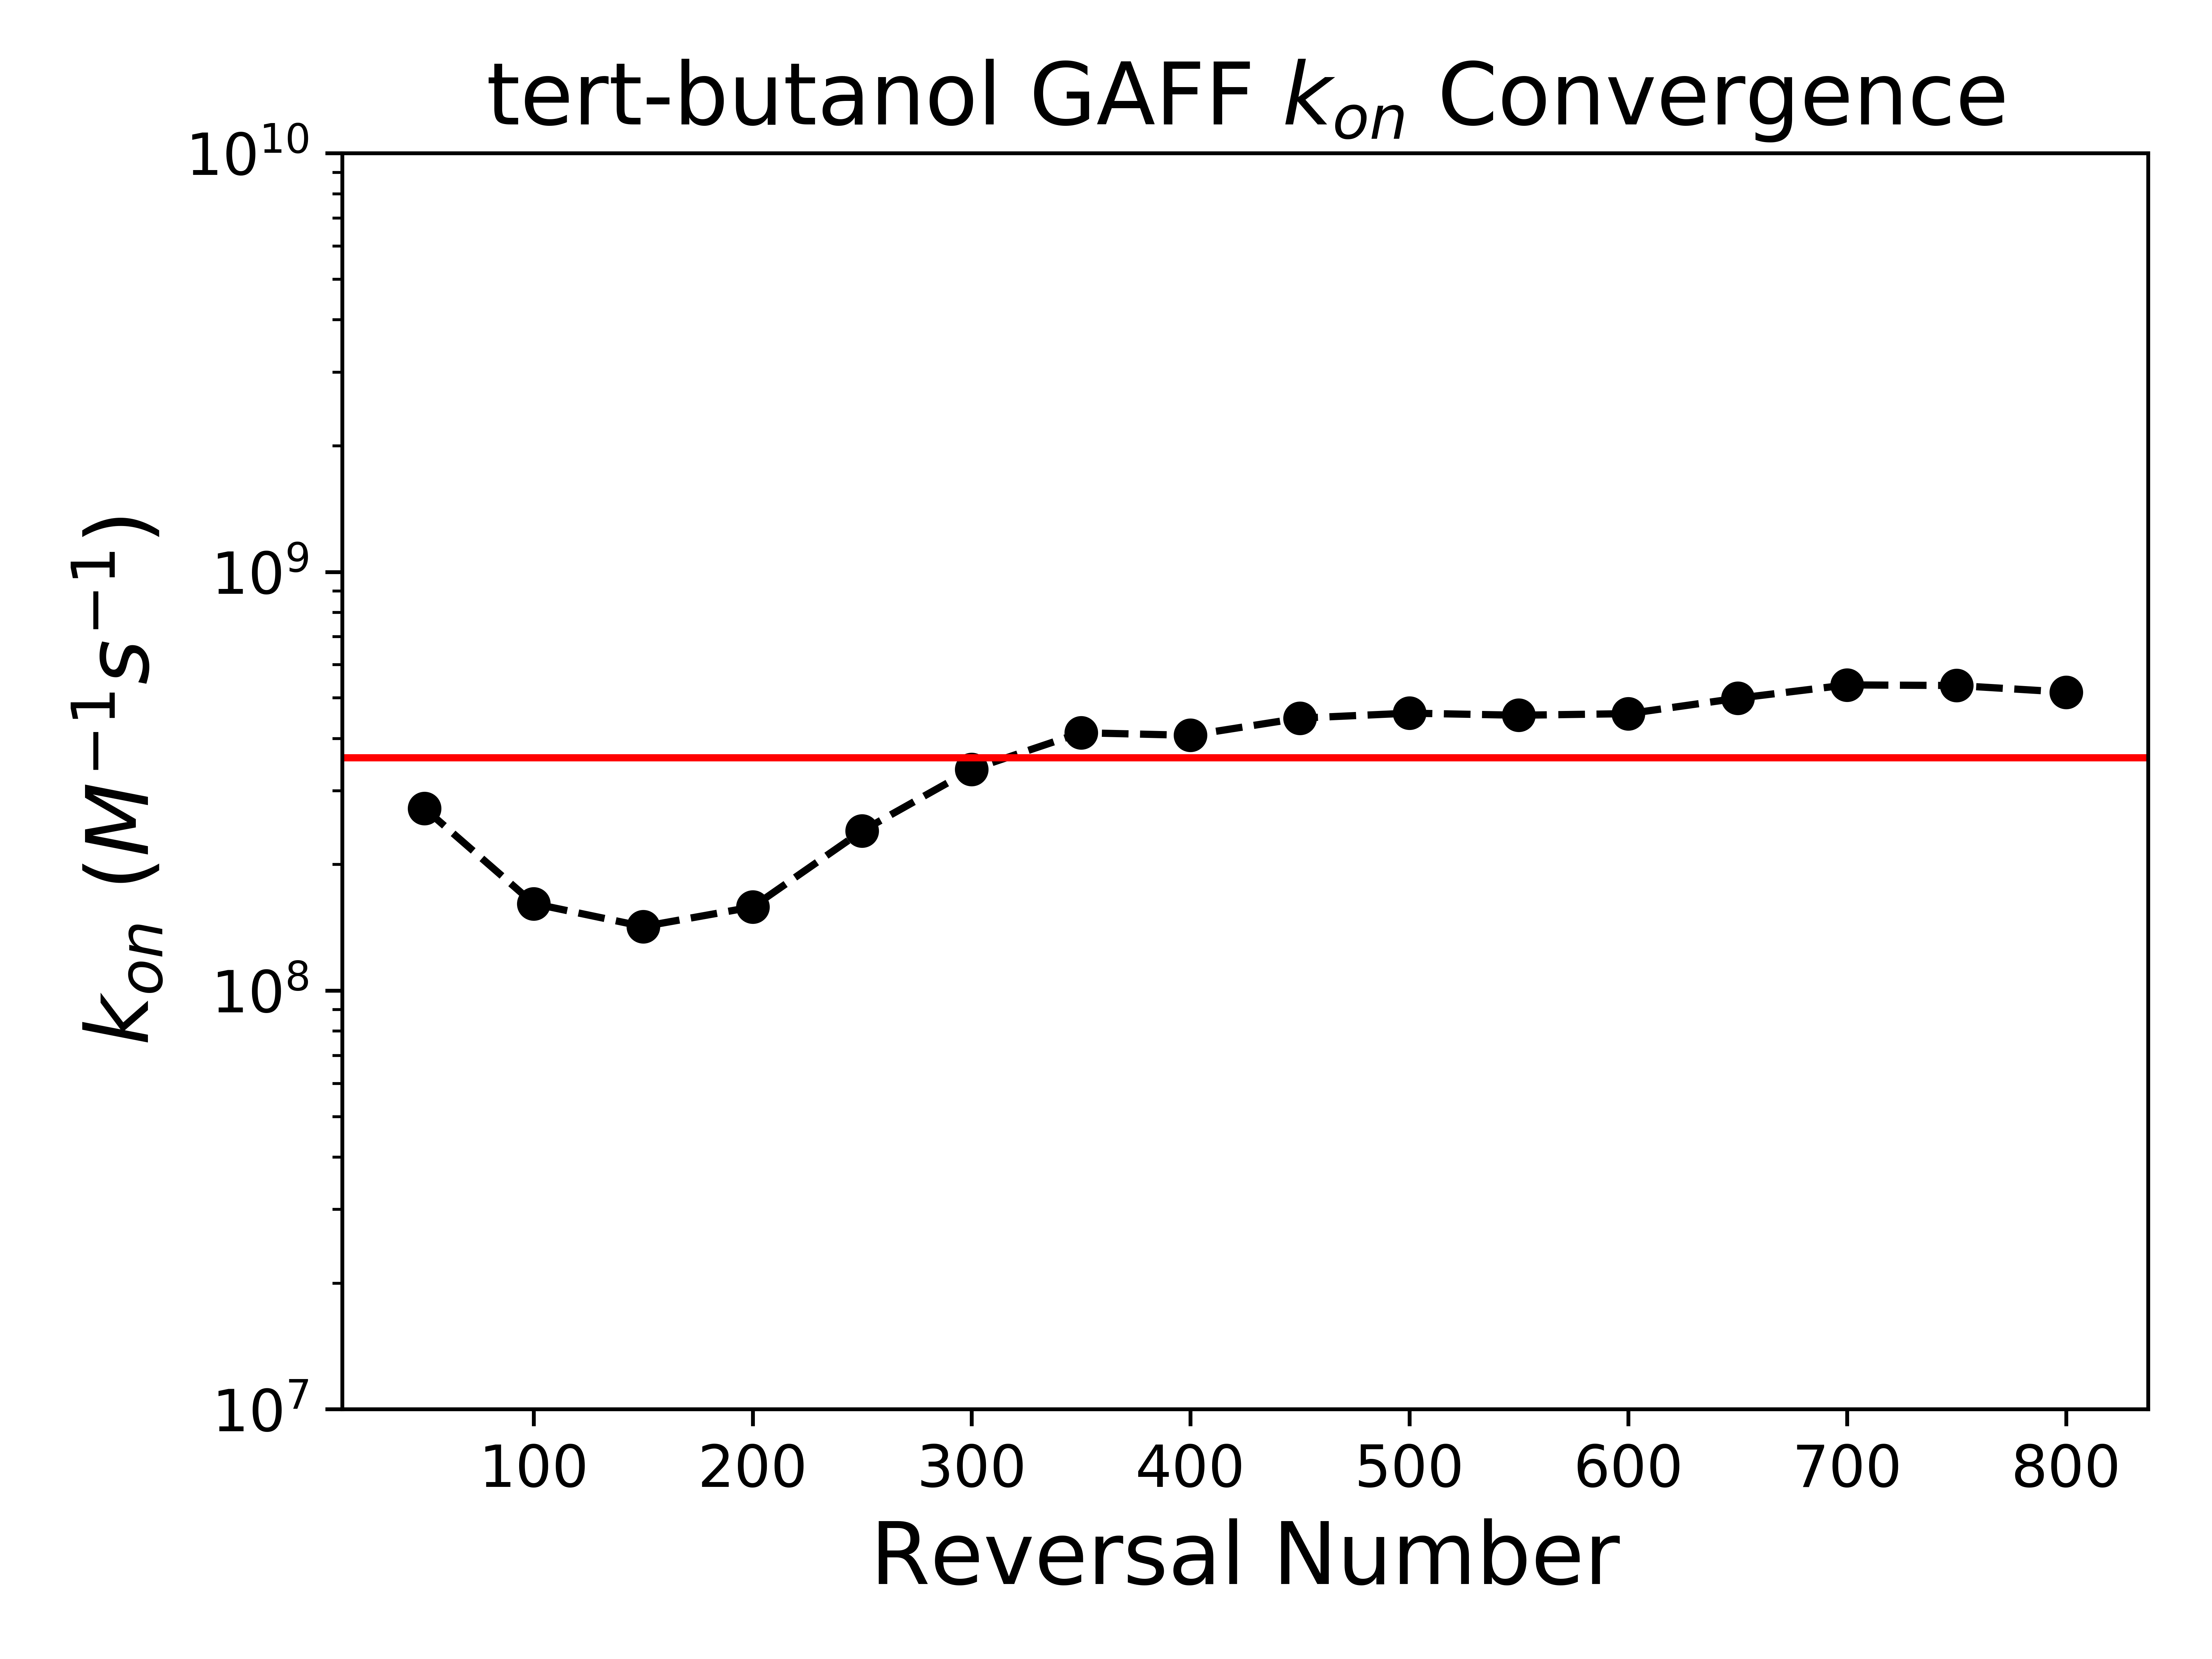
\includegraphics[width=\linewidth]{high_res_images/gaff_rate_conv_images/tert-butanol_gaff_on_conv.png}
	\end{subfigure}
	\begin{subfigure}{0.3\linewidth}
		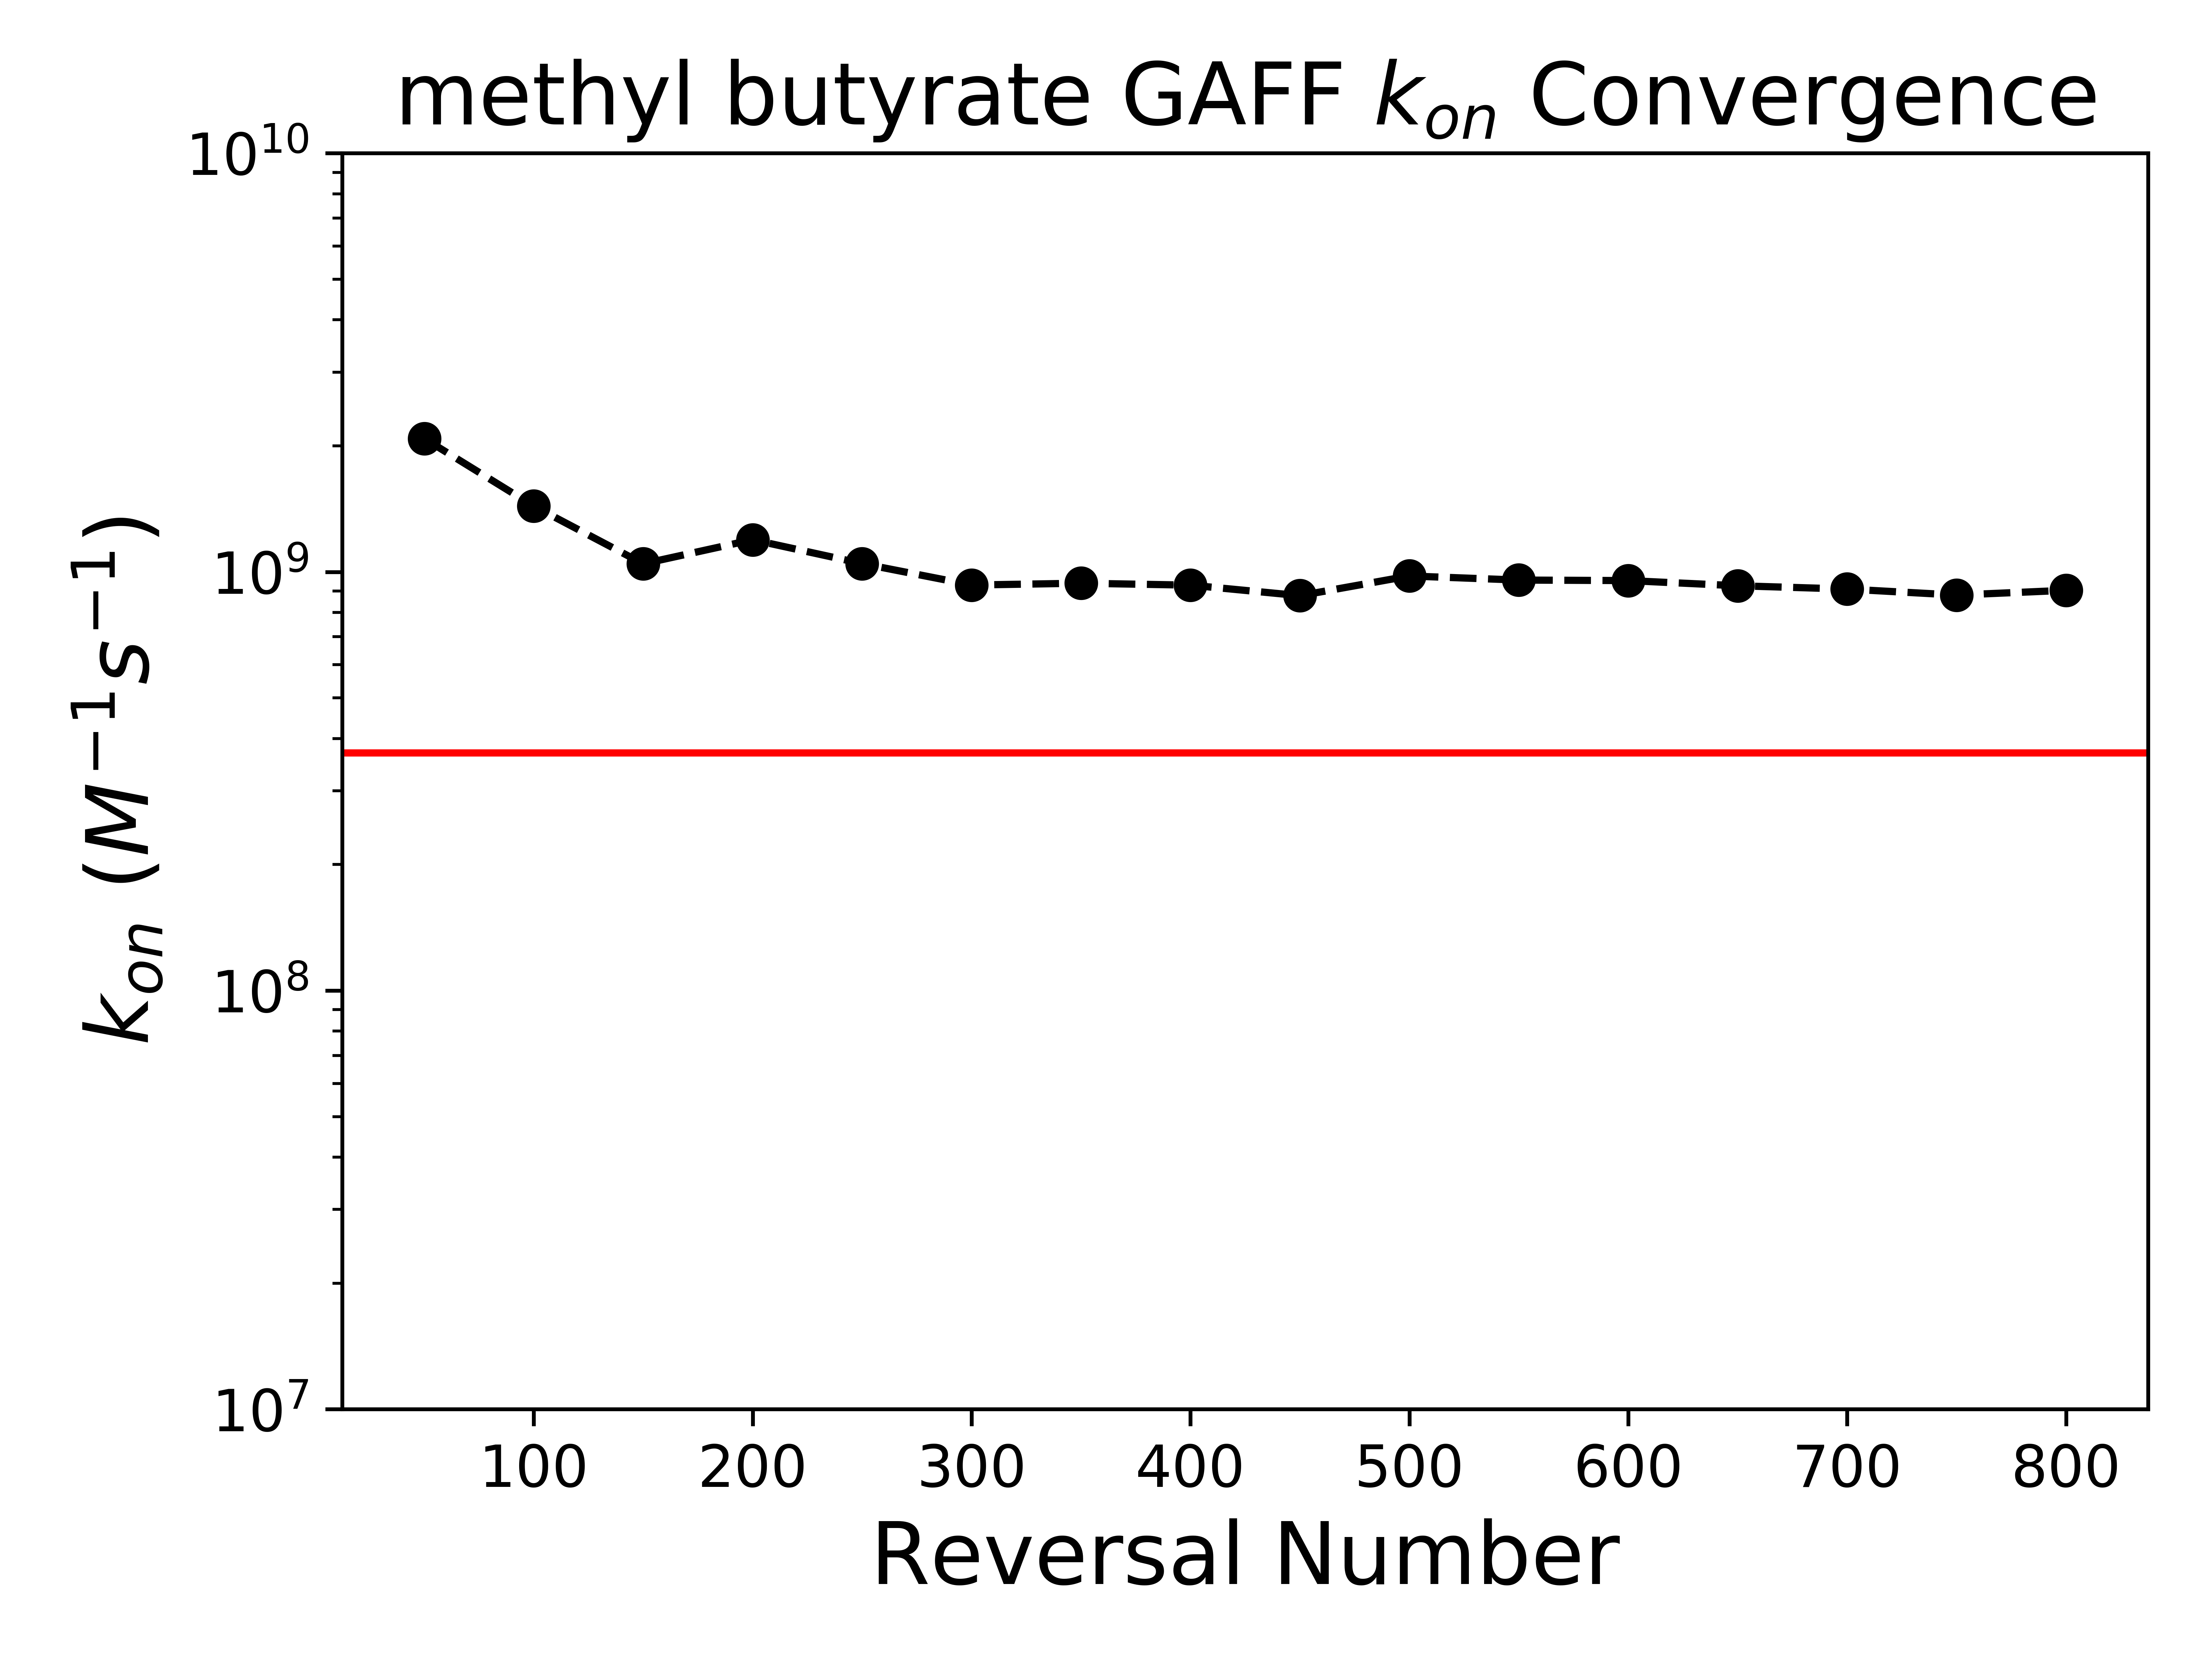
\includegraphics[width=\linewidth]{high_res_images/gaff_rate_conv_images/methylbutyrate_gaff_on_conv.png}
	\end{subfigure}
	\begin{subfigure}{0.3\linewidth}
		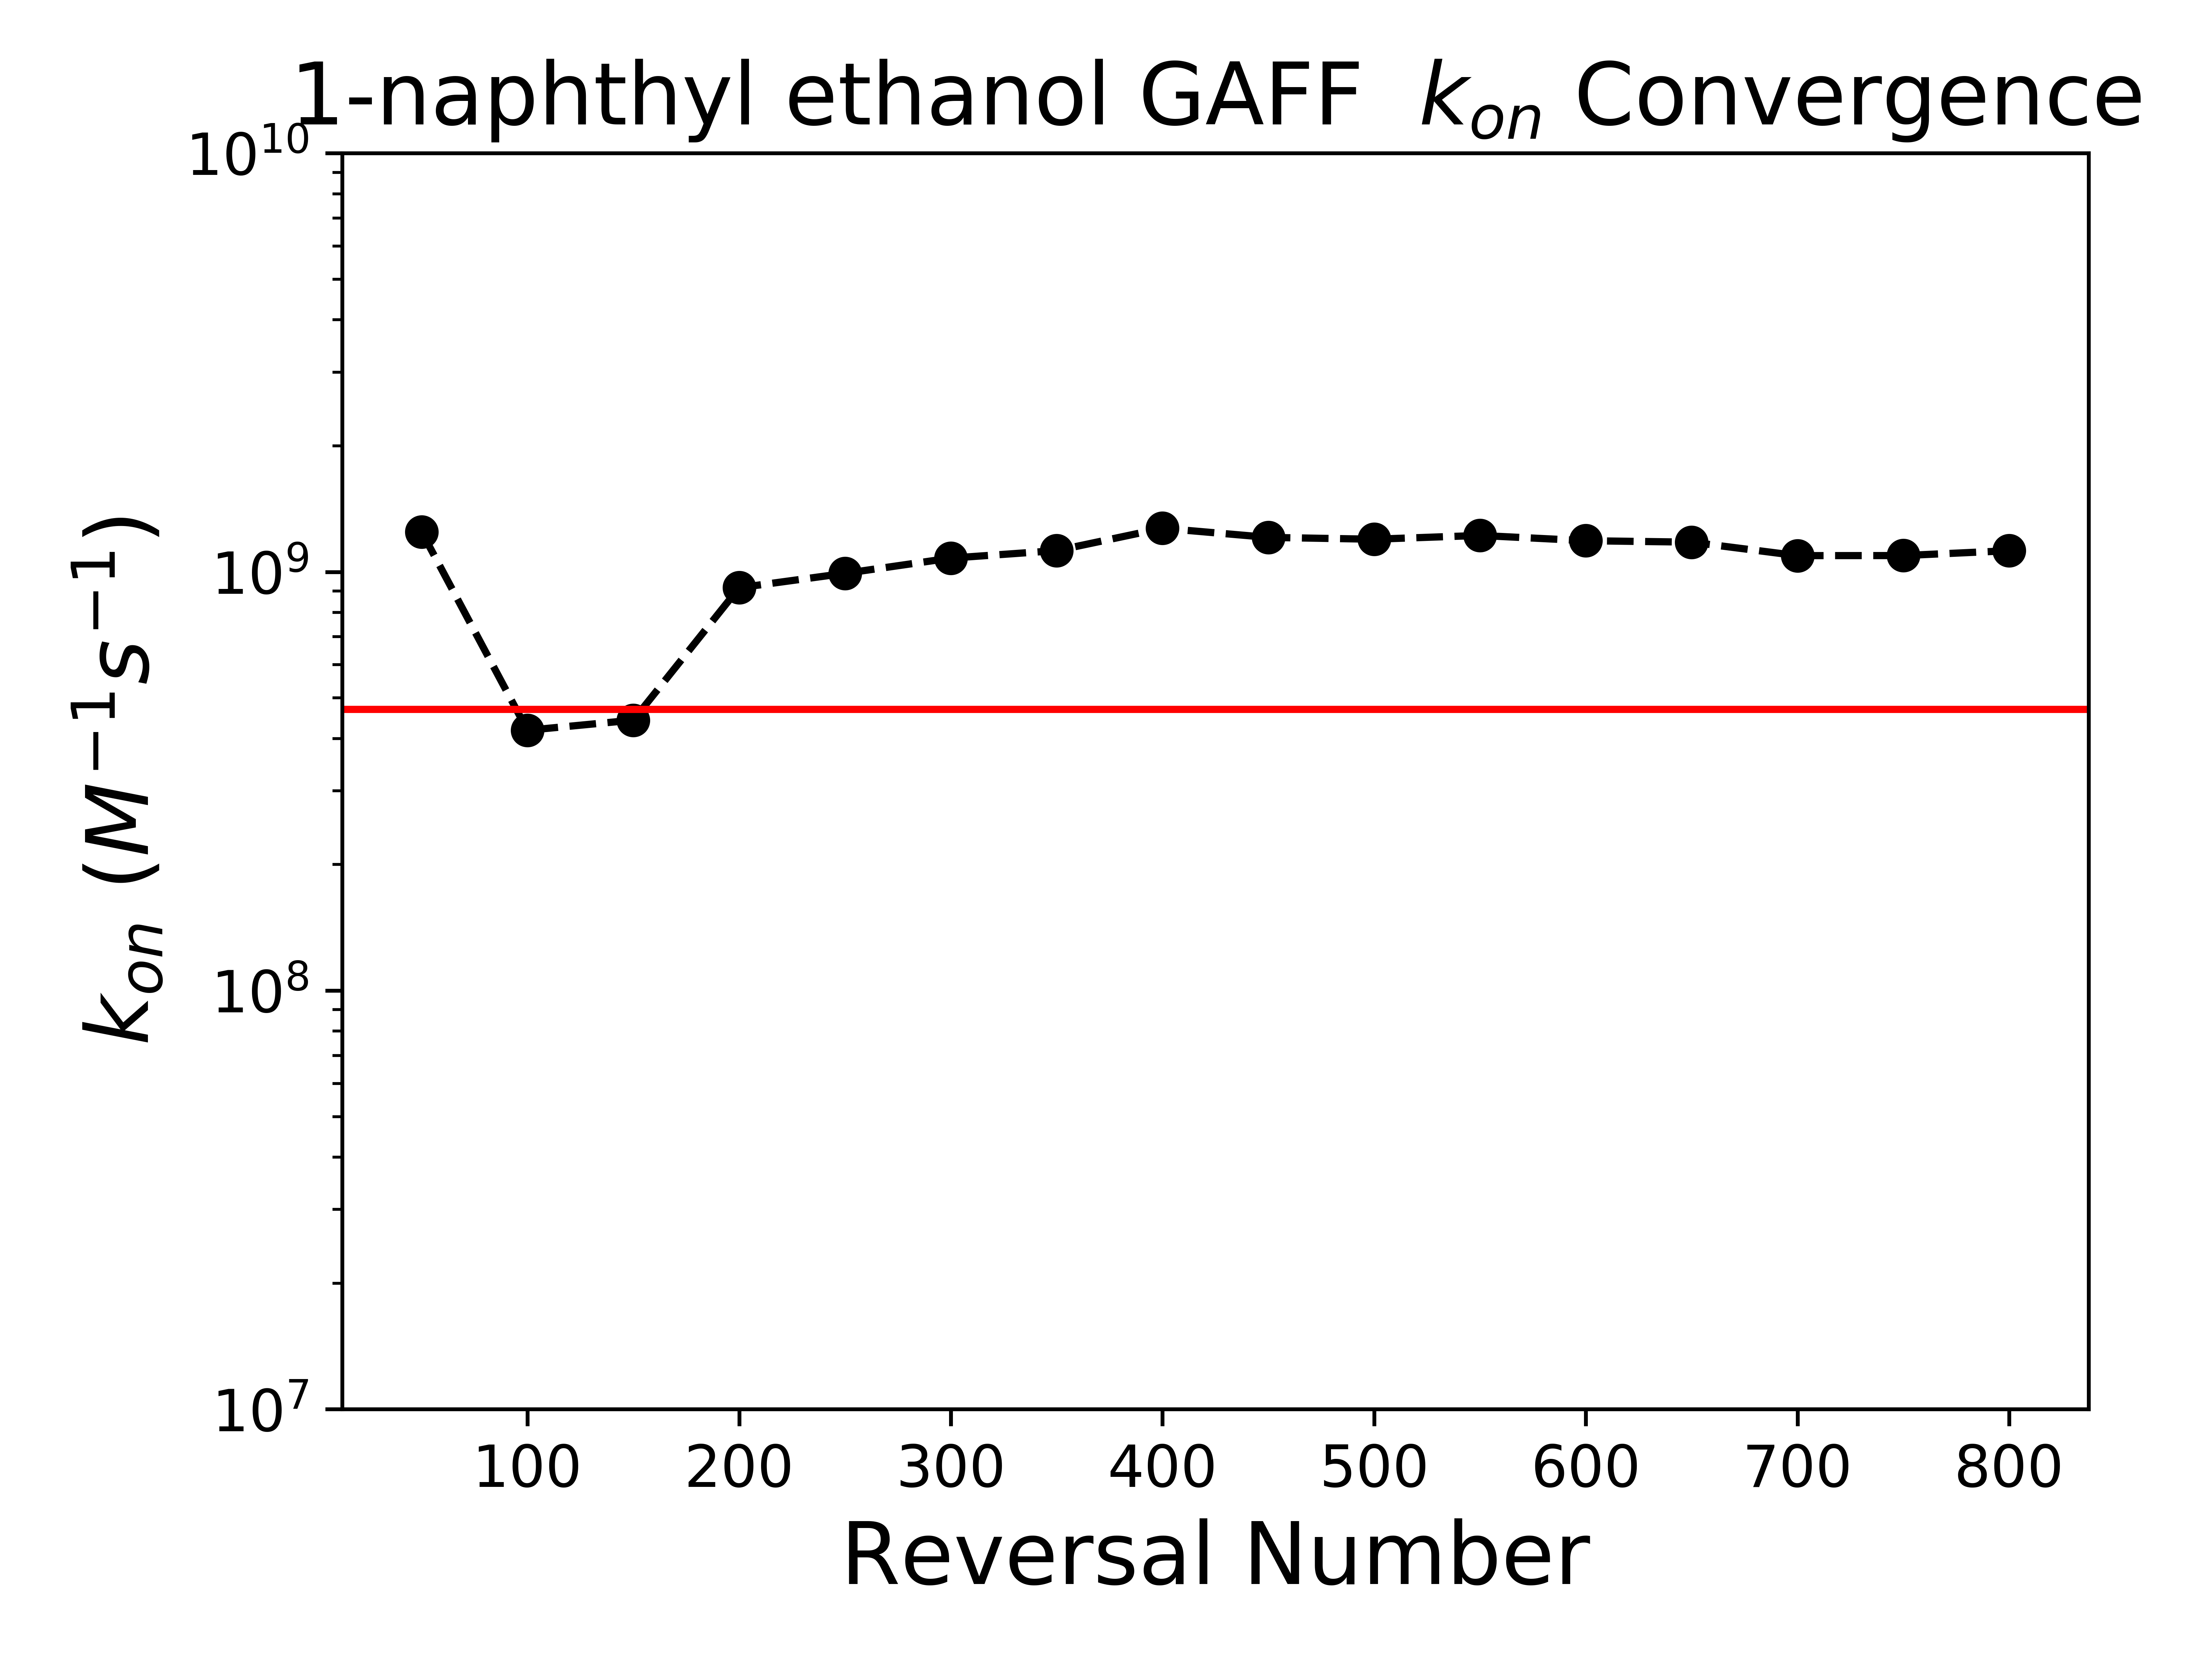
\includegraphics[width=\linewidth]{high_res_images/gaff_rate_conv_images/1-naphthylethanol_gaff_on_conv.png}
	\end{subfigure}
	\begin{subfigure}{0.3\linewidth}
		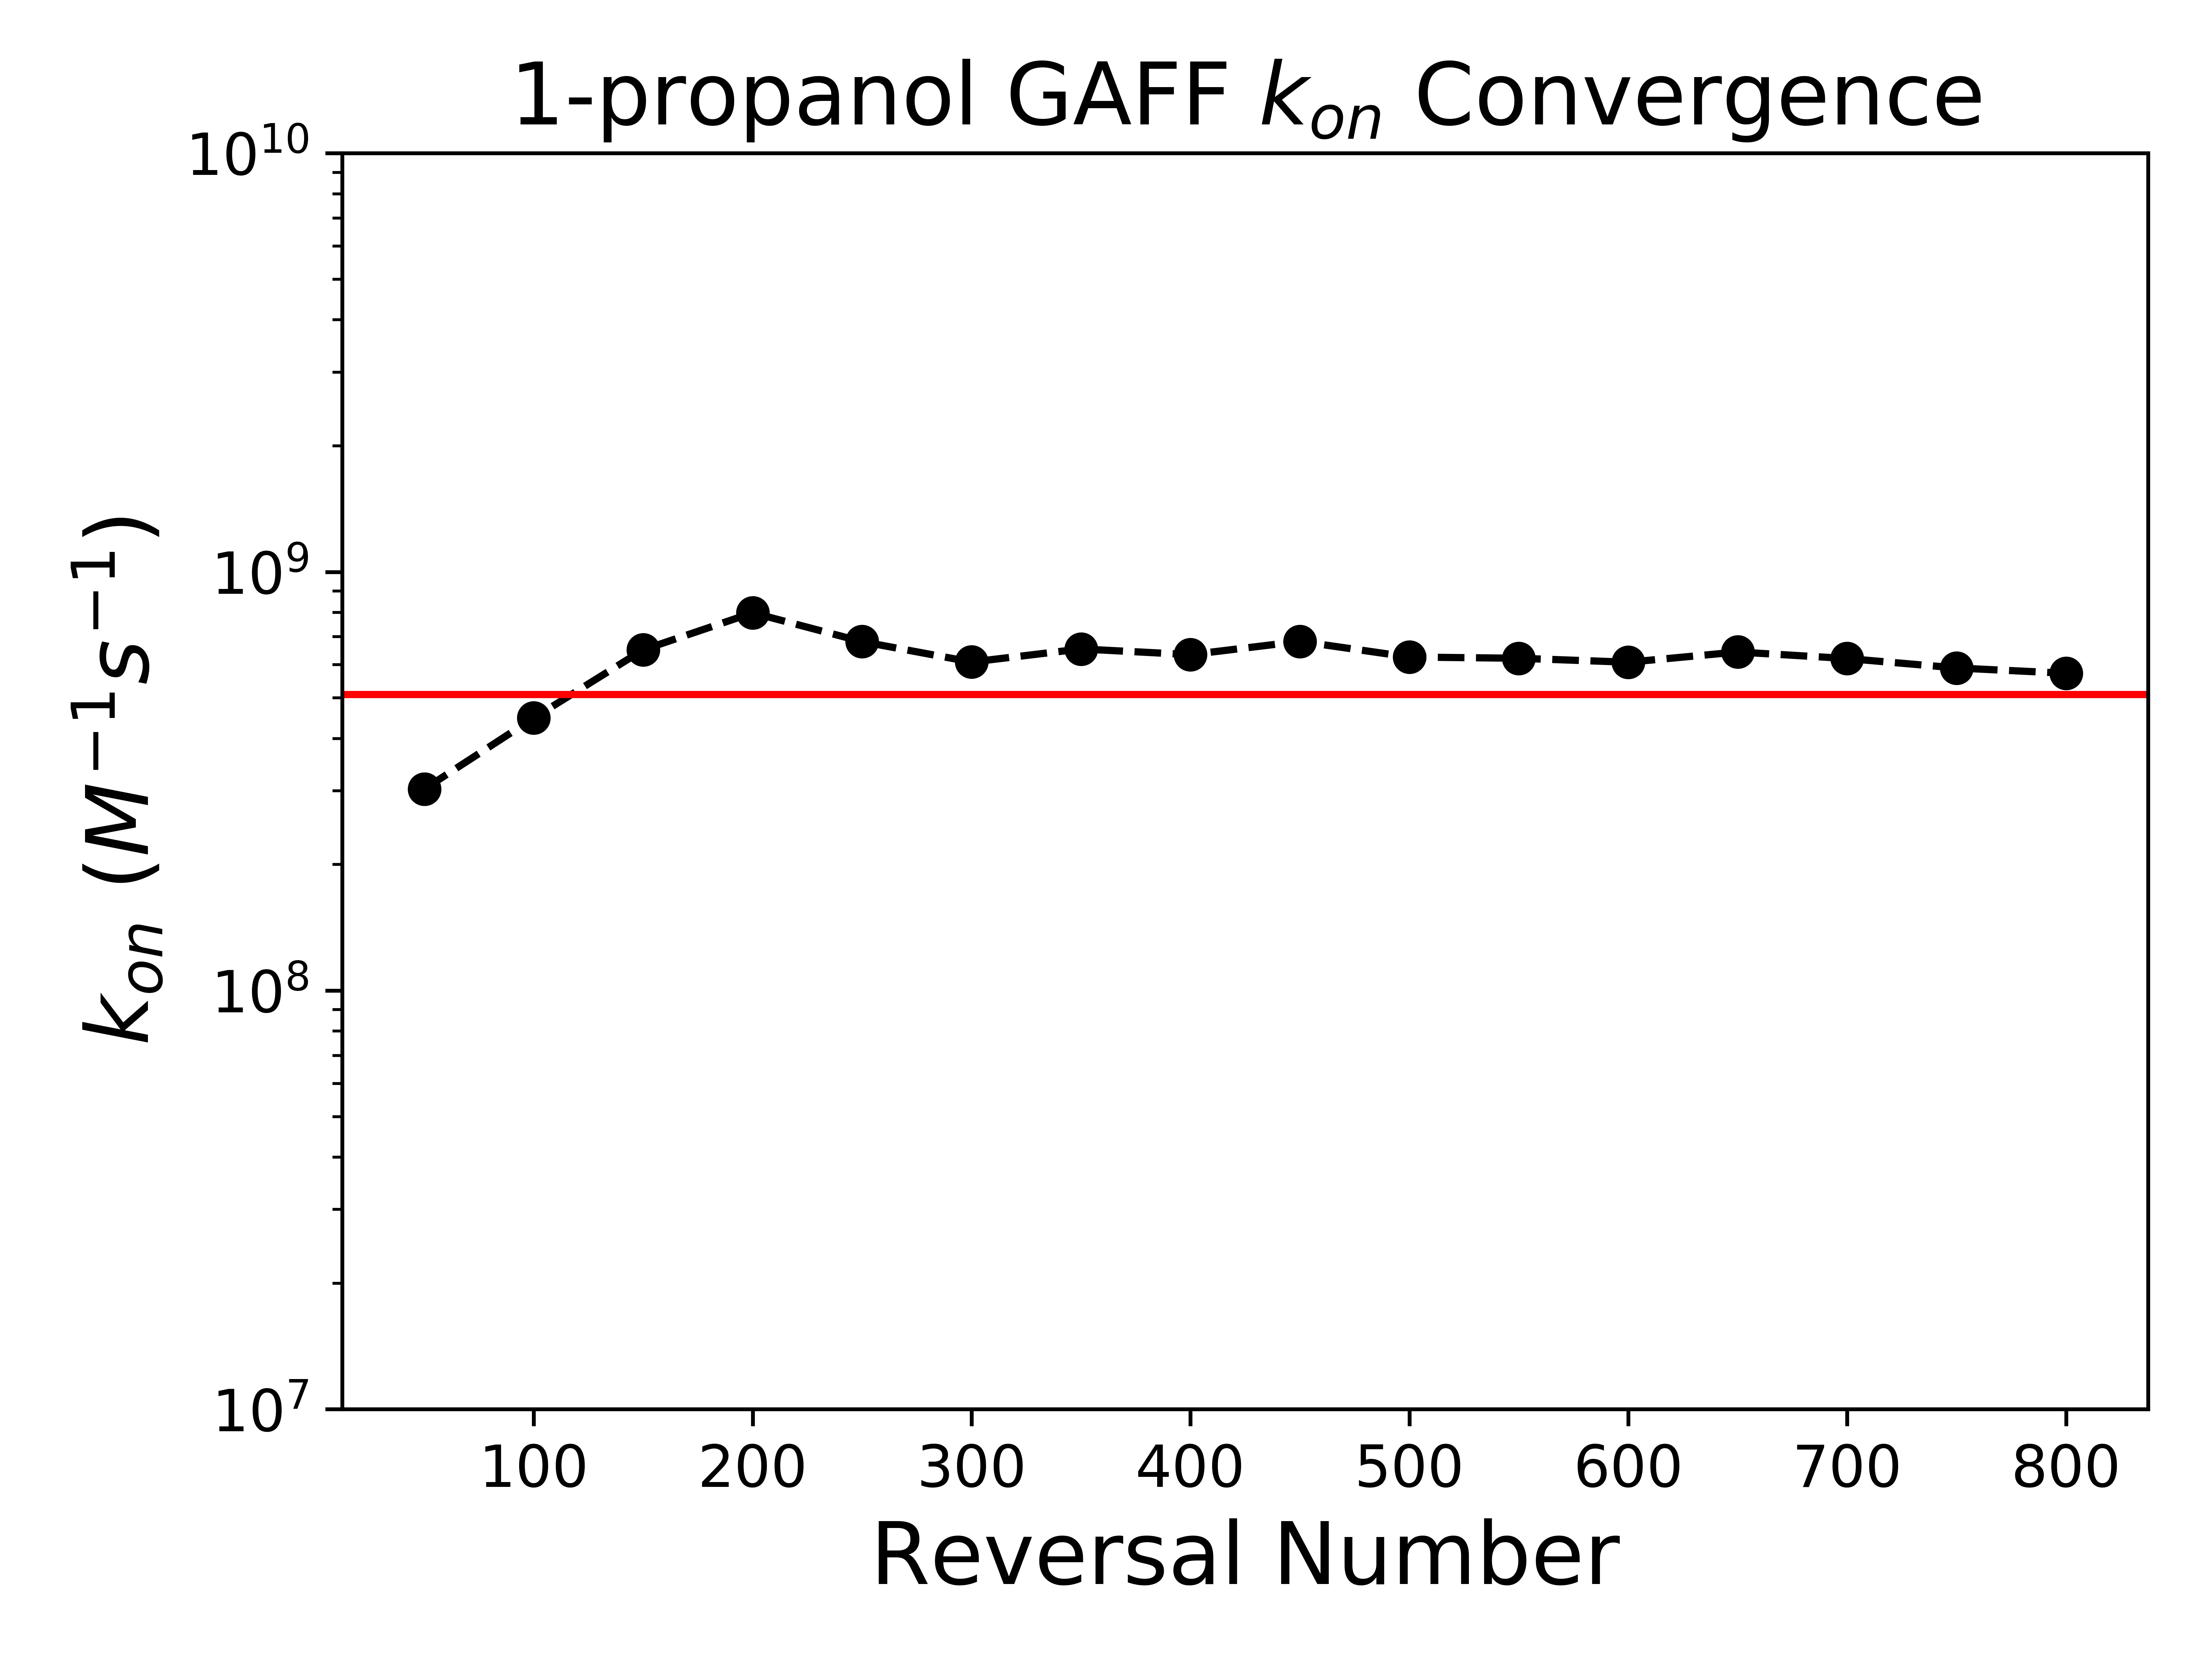
\includegraphics[width=\linewidth]{high_res_images/gaff_rate_conv_images/1-propanol_gaff_on_conv.png}
	\end{subfigure}
	\begin{subfigure}{0.3\linewidth}
		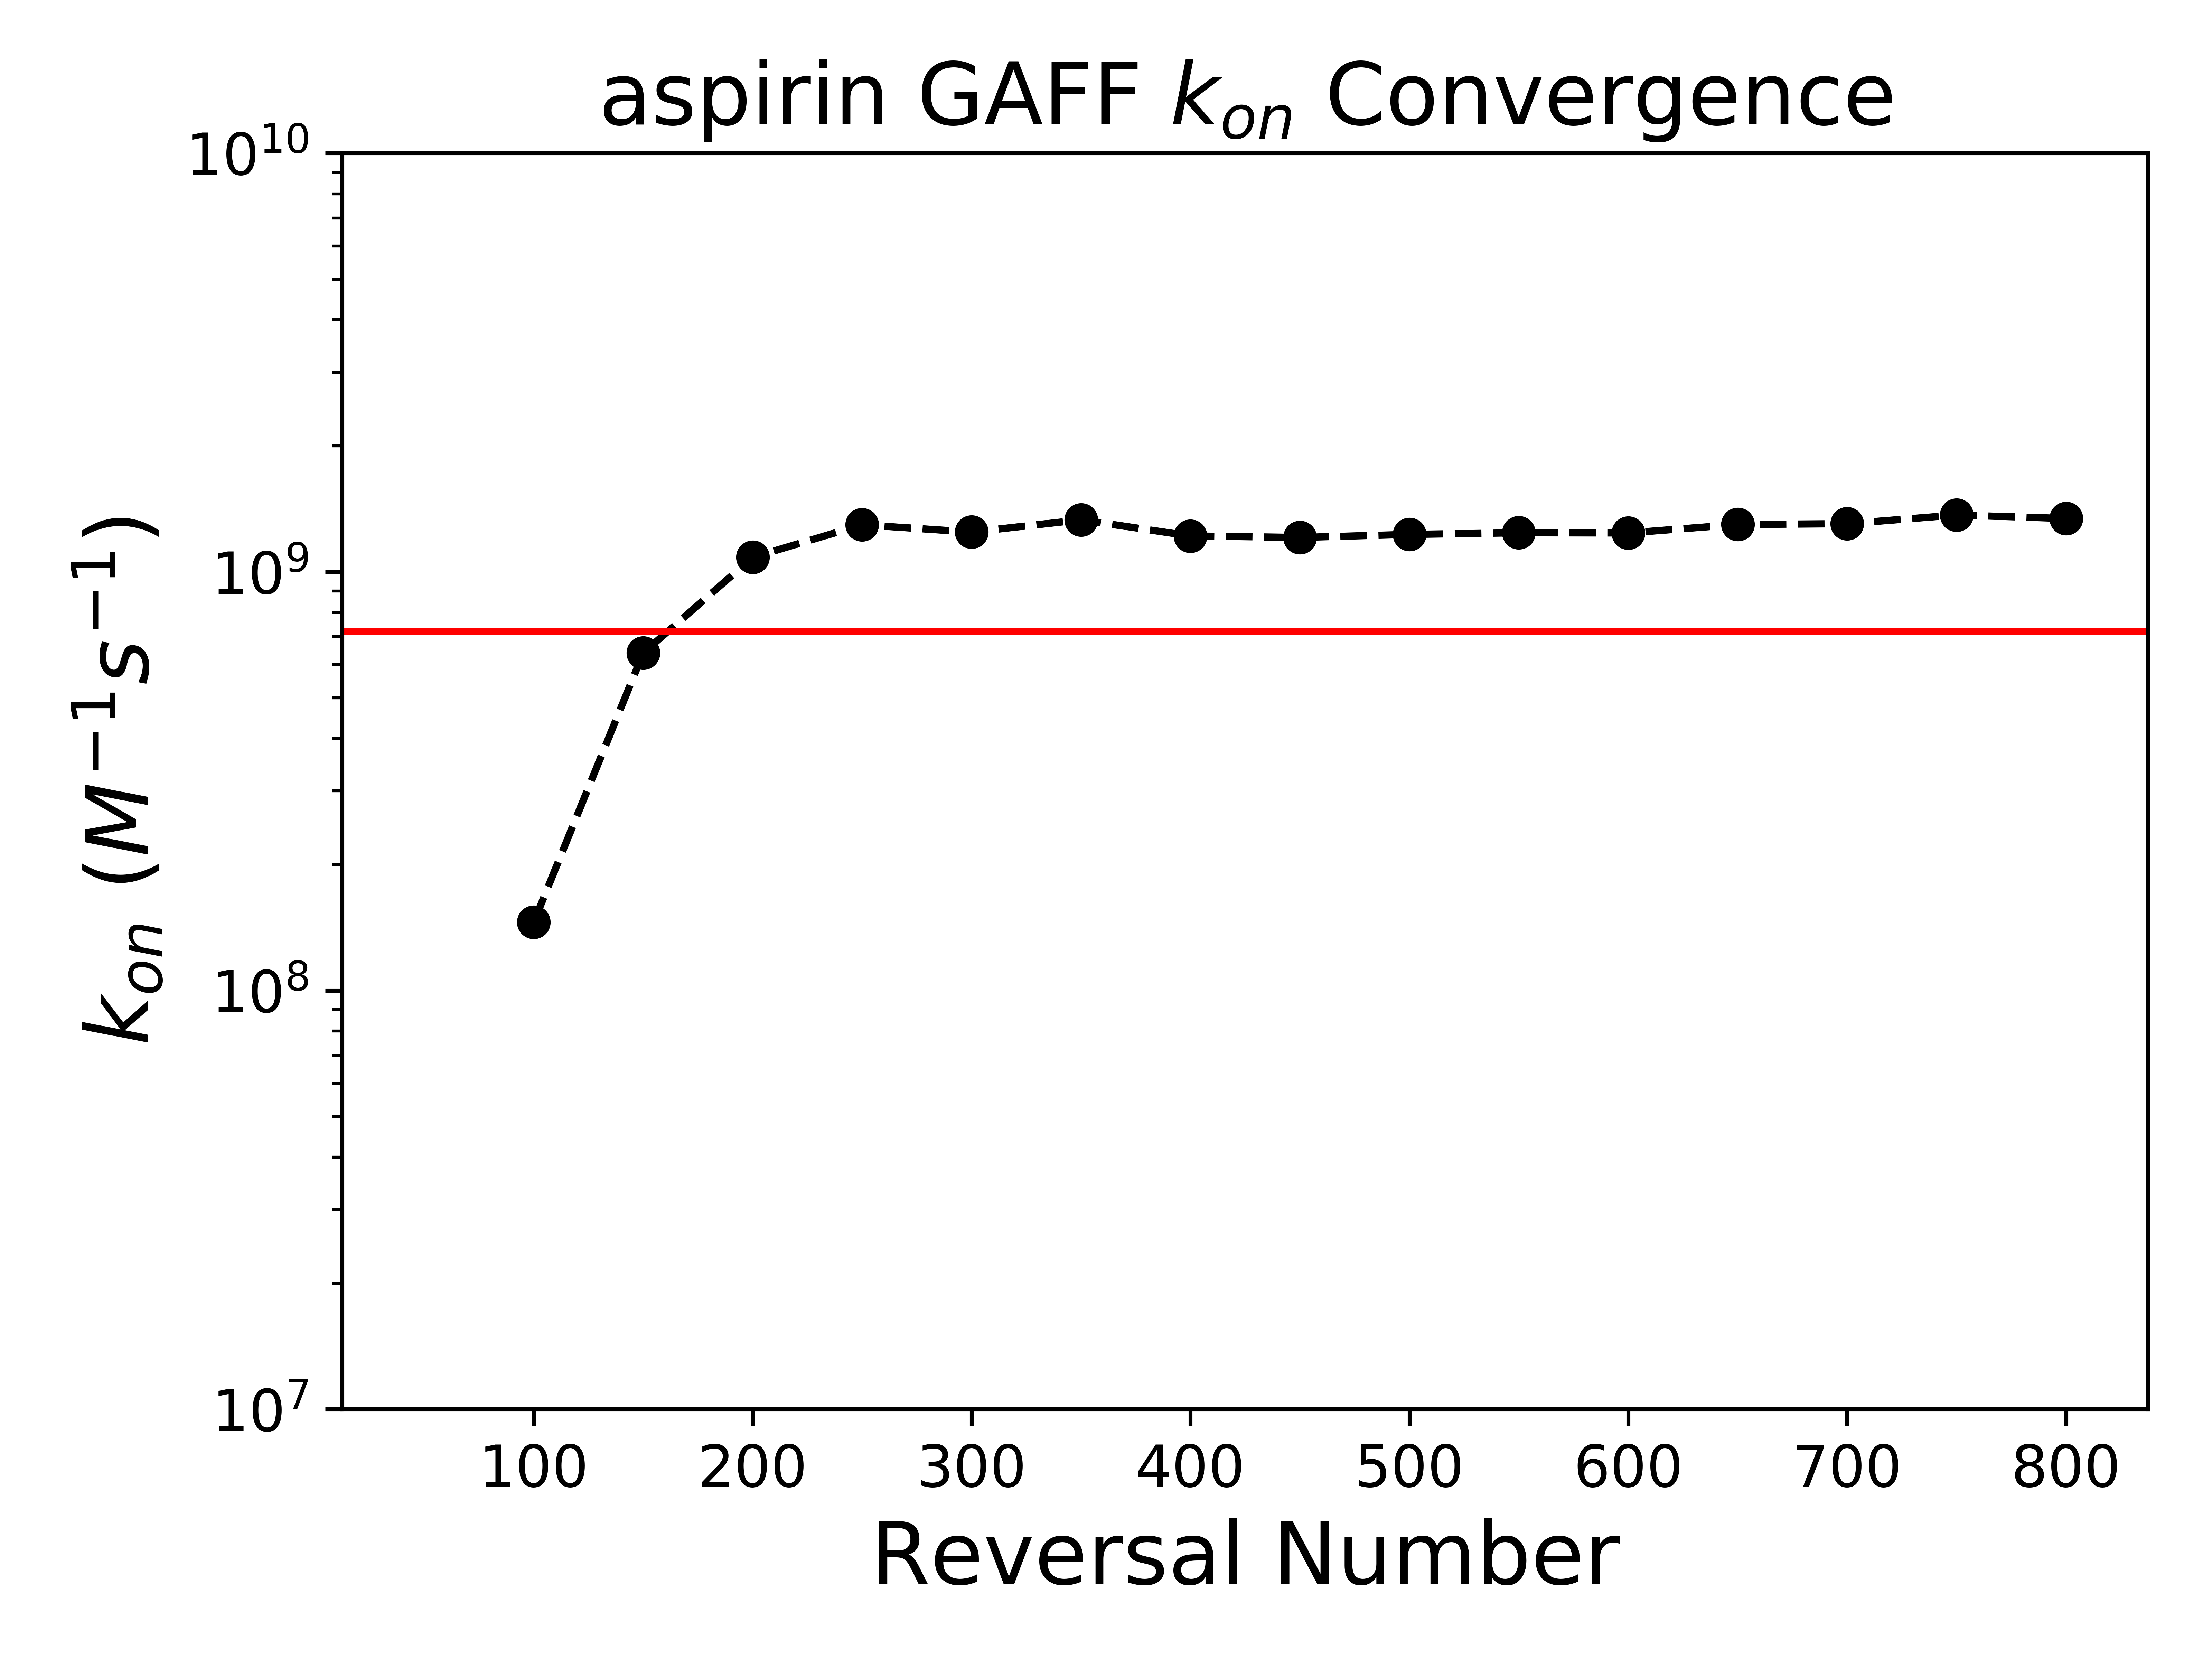
\includegraphics[width=\linewidth]{high_res_images/gaff_rate_conv_images/aspirin_gaff_on_conv.png}
	\end{subfigure}
	\caption{Convergence of on rates as a function of the number of reversals included using the GAFF forcefield}
\end{figure}